\section{Normal Distribution/ Gaussian Distribution (${N}(\mu, \sigma^2)$, ${N}(x|\mu, \sigma^2)$)}


\begin{table}[H]
    \hfill
    \begin{minipage}{0.45\linewidth}
        \begin{figure}[H]
            \centering
            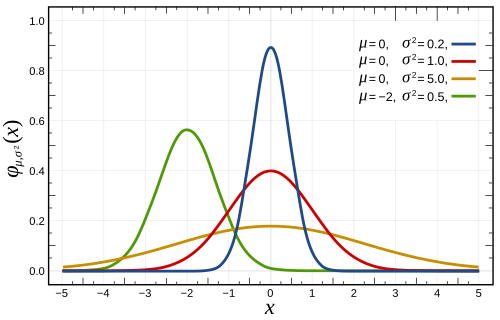
\includegraphics[
                width=\linewidth,
                height=5cm,
                keepaspectratio,
            ]{images/distributions/Normal_Distribution_PDF.svg.png}
            \caption{Normal Distribution: PDF \cite{wiki/Normal_distribution}}
        \end{figure}
    \end{minipage}
    \hfill
    \begin{minipage}{0.45\linewidth}
        \begin{figure}[H]
            \centering
            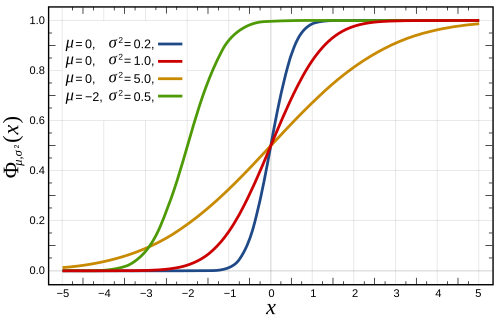
\includegraphics[
                width=\linewidth,
                height=5cm,
                keepaspectratio,
            ]{images/distributions/Normal_Distribution_CDF.svg.png}
            \caption{Normal Distribution: CDF \cite{wiki/Normal_distribution}}
        \end{figure}
    \end{minipage}
    \hfill
\end{table}

\begin{enumerate}
    \item Denoted by: $\mathcal{N}(\mu, \sigma^2)$
\end{enumerate}


\subsection{PDF ($f_{\mu, \sigma}(x)$ or $f(x|\mu, \sigma)$)}

\begin{enumerate}
    \item  $
        f_{\mu, \sigma}(x)
        = \dfrac{1}{\sigma\sqrt{2\pi}} \exp\dParenBrac{-\dfrac{(x-\mu)^2}{2\sigma^2}}
    $
    \hfill \cite{statistics/book/Statistics-for-Data-Scientists/Maurits-Kaptein}
    \begin{enumerate}
        \item[] $\mu \in \mbbR$: indicates the mean value of the population of the variable of interest
        \hfill \cite{statistics/book/Statistics-for-Data-Scientists/Maurits-Kaptein}

        \item[] $\sigma \in \mbbR$: indicates the standard deviation ($\sigma^2 > 0$)
        \hfill \cite{statistics/book/Statistics-for-Data-Scientists/Maurits-Kaptein}
    \end{enumerate}

    \item $f_{\mu, \sigma}(x) = \dfrac{1}{\sigma}\phi\dParenBrac{\dfrac{x-\mu}{\sigma}}$
    \hfill \cite{statistics/book/Statistics-for-Data-Scientists/Maurits-Kaptein}


    \item it can be used to approximate other PDFs when the sample size or the size of the data is getting large.
    \hfill \cite{statistics/book/Statistics-for-Data-Scientists/Maurits-Kaptein}

    \item This has the advantage that important features of the normal density function can be transferred to other densities when the approximation is quite close.
    \hfill \cite{statistics/book/Statistics-for-Data-Scientists/Maurits-Kaptein}

    \item The shape of the normal PDF is equal to the famous “bell-shape” curve
    \hfill \cite{statistics/book/Statistics-for-Data-Scientists/Maurits-Kaptein}

    \item areas under the curve:
    \begin{enumerate}
        \item $99.73\%$ of all the population values fall within the interval $[\mu - 3\sigma, \mu + 3\sigma]$
        \hfill \cite{statistics/book/Statistics-for-Data-Scientists/Maurits-Kaptein}

        \item $95.45\%$ of all the population values fall within the interval $[\mu - 2\sigma, \mu + 2\sigma]$ or
        \hfill \cite{statistics/book/Statistics-for-Data-Scientists/Maurits-Kaptein}
        \\[0.2cm]
        .\hfill
        $
            \dint_{\mu - 2\sigma}^{\mu + 2\sigma}
            \phi\dParenBrac{\dfrac{x-\mu}{\sigma}} dx
            =
            \dint_{-2}^{2}
            \phi(x) dx
            =
            0.9545
        $
        \hfill \cite{statistics/book/Statistics-for-Data-Scientists/Maurits-Kaptein}

        \item $95\%$ of the values fall within $[\mu - 1.96\sigma, \mu + 1.96\sigma]$
        \hfill \cite{statistics/book/Statistics-for-Data-Scientists/Maurits-Kaptein}
    \end{enumerate}

    \item  describes both positive and negative values
    \hfill \cite{statistics/book/Statistics-for-Data-Scientists/Maurits-Kaptein}

    \item a random measurement error that could be described by a normal PDF is more likely to be closer to zero than to be further away from zero (due to the bell shape of the density).
    \hfill \cite{statistics/book/Statistics-for-Data-Scientists/Maurits-Kaptein}
\end{enumerate}









\subsection{Maximum Likelihood}

\begin{enumerate}
    \item If our data set $\bm{x}$ is i.i.d., then we can therefore write the probability of the data set, given $\mu$  and $\sigma^2$, in the form
    \hfill \cite{ml/book/Pattern-Recognition-And-Machine-Learning/Christopher-M-Bishop}
    \\
    .\hfill
    $
        P(\bm{x}|\mu , \sigma^2)
        = \dprod^{N}_{n=1} \mathcal{N} (x_n|\mu , \sigma^2)
    $
    \hfill \cite{ml/book/Pattern-Recognition-And-Machine-Learning/Christopher-M-Bishop}

    \item Log likelihood function:
    \hfill \cite{ml/book/Pattern-Recognition-And-Machine-Learning/Christopher-M-Bishop}
    \\
    .\hfill
    $
        \ln (p (\bm{x}|\mu , \sigma ^2))
        = - \dfrac{1}{2\sigma ^2} \dsum^N_{n=1} (x_n - \mu )^2 - \dfrac{N }{2} \ln (\sigma ^2) - \dfrac{N }{2} \ln(2\pi)
    $
    \hfill \cite{ml/book/Pattern-Recognition-And-Machine-Learning/Christopher-M-Bishop}

    \item Maximizing $\ln (p (\bm{x}|\mu , \sigma ^2))$ with respect to $\mu$, we obtain the maximum likelihood solution given by
    $
        \mu_{ML}
        = \dfrac{1}{N} \dsum_{n=1}^N x_n
    $
    which is the sample mean, i.e., the mean of the observed values $\dCurlyBrac{x_n}$.
    \hfill \cite{ml/book/Pattern-Recognition-And-Machine-Learning/Christopher-M-Bishop}

    \item Maximizing $\ln (p (\bm{x}|\mu , \sigma ^2))$ with respect to $\sigma^2$, we obtain the maximum likelihood solution for the variance in the form
    $
        \sigma^2 _{ML} = \dfrac{1}{N} \dsum^N _{n=1} (x_n - \mu _{ML})^2
    $
    which is the sample variance measured with respect to the sample mean $\mu _{ML}$.
    \hfill \cite{ml/book/Pattern-Recognition-And-Machine-Learning/Christopher-M-Bishop}

    \item
    $\mbbE[\mu _{ML}] = \mu $
    \hfill
    $\mbbE[\sigma ^2_{ML}] = \dParenBrac{\dfrac{N - 1}{N}} \sigma ^2$
    \hfill \cite{ml/book/Pattern-Recognition-And-Machine-Learning/Christopher-M-Bishop}
\end{enumerate}







\subsection{Summary}

\begin{enumerate}

    \item
    \textbf{Notation}:
    $
        {\displaystyle {\mathcal {N}}(\mu ,\sigma ^{2})}
    $
    \hfill \cite{wiki/Normal_distribution}

    \item
    \textbf{Parameters}:
    \begin{enumerate}
        \item ${\displaystyle \mu \in \mathbb {R} }$ = mean (location)
        \hfill \cite{wiki/Normal_distribution}

        \item ${\displaystyle \sigma ^{2}\in \mathbb {R} _{>0}}$ = variance (squared scale)
        \hfill \cite{wiki/Normal_distribution}
    \end{enumerate}

    \item
    \textbf{Support/ Rand Var}:
    $x \in \mbbR$
    \hfill \cite{wiki/Normal_distribution}

    \item
    \textbf{PDF}:
    $ {\displaystyle {\dfrac {1}{\sqrt {2\pi \sigma ^{2}}}}e^{-{\dfrac {(x-\mu )^{2}}{2\sigma ^{2}}}}} $
    \hfill\cite{wiki/Normal_distribution}

    \item
    \textbf{CDF}:
    $ {\displaystyle \Phi \left({\dfrac {x-\mu }{\sigma }}\right)={\dfrac {1}{2}}\left[1+\operatorname {erf} \left({\dfrac {x-\mu }{\sigma {\sqrt {2}}}}\right)\right]} $
    \hfill\cite{wiki/Normal_distribution}

    \item
    \textbf{Quantile}:
    $ {\displaystyle \mu +\sigma {\sqrt {2}}\operatorname {erf} ^{-1}(2p-1)} $
    \hfill\cite{wiki/Normal_distribution}

    \item
    \textbf{Mean}:
    $ {\displaystyle \mu } $
    \hfill\cite{wiki/Normal_distribution}

    \item
    \textbf{Median}:
    $ {\displaystyle \mu } $
    \hfill\cite{wiki/Normal_distribution}

    \item
    \textbf{Mode}:
    $ {\displaystyle \mu } $
    \hfill\cite{wiki/Normal_distribution}

    \item
    \textbf{Variance}:
    $ {\displaystyle \sigma ^{2}} $
    \hfill\cite{wiki/Normal_distribution}

    \item
    \textbf{Precision}: $\beta = \dfrac{1}{\sigma^2}$
    \hfill \cite{ml/book/Pattern-Recognition-And-Machine-Learning/Christopher-M-Bishop}

    \item
    \textbf{Median absolute deviation (MAD)}:
    $ {\displaystyle \sigma {\sqrt {2}}\,\operatorname {erf} ^{-1}(1/2)} $
    \hfill\cite{wiki/Normal_distribution}

    \item
    \textbf{Average absolute deviation (AAD)}:
    $ {\textstyle \sigma {\sqrt {2/\pi }}} $
    \hfill\cite{wiki/Normal_distribution}

    \item
    \textbf{Skewness}: $0$
    \hfill\cite{wiki/Normal_distribution}

    \item
    \textbf{Excess kurtosis}: $0$
    \hfill\cite{wiki/Normal_distribution}

    \item
    \textbf{Entropy}: $ {\textstyle {\dfrac {1}{2}}\log(2\pi e\sigma ^{2})} $
    \hfill\cite{wiki/Normal_distribution}

    \item
    \textbf{Moment-generating function (MGF)}: $ {\displaystyle \exp(\mu t+\sigma ^{2}t^{2}/2)} $
    \hfill\cite{wiki/Normal_distribution}

    \item
    \textbf{Characteristic function (CF)}: $ {\displaystyle \exp(i\mu t-\sigma ^{2}t^{2}/2)} $
    \hfill\cite{wiki/Normal_distribution}

    \item
    \textbf{Fisher information}:
    \begin{enumerate}
        \item ${\displaystyle {\mathcal {I}}(\mu ,\sigma )={\begin{pmatrix}1/\sigma ^{2}&0\\0&2/\sigma ^{2}\end{pmatrix}}}$

        \item ${\displaystyle {\mathcal {I}}(\mu ,\sigma ^{2})={\begin{pmatrix}1/\sigma ^{2}&0\\0&1/(2\sigma ^{4})\end{pmatrix}}}$
    \end{enumerate}
    \hfill\cite{wiki/Normal_distribution}

    \item
    \textbf{Kullback–Leibler divergence}:
    ${\displaystyle D_{KL} = {1 \over 2}\left\{\left({\dfrac {\sigma _{0}}{\sigma _{1}}}\right)^{2}+{\dfrac {(\mu _{1}-\mu _{0})^{2}}{\sigma _{1}^{2}}}-1+\ln {\sigma _{1}^{2} \over \sigma _{0}^{2}}\right\}}$
    \hfill\cite{wiki/Normal_distribution}

    \item
    \textbf{Expected shortfall}:
    ${\displaystyle \mu +\sigma {\dfrac {{\dfrac {1}{\sqrt {2\pi }}}e^{\dfrac {-\left(q_{p}\left({\dfrac {X-\mu }{\sigma }}\right)\right)^{2}}{2}}}{1-p}}}$
    \hfill\cite{wiki/Normal_distribution}

    \item
    \textbf{second order moment}:
    $
        \mbbE[x^2]
        = \dint_{-\infty}^\infty \mathcal{N}(x|\mu, \sigma^2) x^2 dx
        = \mu^2 + \sigma^2
    $
    \hfill \cite{ml/book/Pattern-Recognition-And-Machine-Learning/Christopher-M-Bishop}

\end{enumerate}









\subsection{Normally Distributed Populations}

\begin{enumerate}
    \item we assume that the random variables $X_1 , X_2, \cdots , X_ n$ are i.i.d. normally distributed, $X _i \sim \mathcal{N} (\mu, \sigma^ 2)$
    \hfill \cite{statistics/book/Statistics-for-Data-Scientists/Maurits-Kaptein}

    \item \textbf{Properties}:
    \begin{enumerate}
        \item \textbf{Property 1}:
        \hfill \cite{statistics/book/Statistics-for-Data-Scientists/Maurits-Kaptein}
        \begin{enumerate}
            \item The sum of the random variables $\dsum^n _{i=1} X_ i$ is again \textbf{normally distributed}, but now with mean $n\mu$ and variance $n\sigma  ^2$ .
            \hfill \cite{statistics/book/Statistics-for-Data-Scientists/Maurits-Kaptein}

            \item Thus this implies that the sample average $\bar{X}$ has a normal distribution with mean $\mu$ and variance $\sigma ^ 2/n$ and thus has $\dfrac{\bar{X} - \mu}{\sigma /\sqrt{n}}$, a standard normal distribution function.
            \hfill \cite{statistics/book/Statistics-for-Data-Scientists/Maurits-Kaptein}
        \end{enumerate}

        \item \textbf{Property 2}:
        \begin{enumerate}
            \item The sum of the squared standardized random variables $\dfrac{1}{\sigma ^2} \dsum^n _{i=1} (X _i - \mu)^2$ is known to be \textbf{chi-square distributed} with $n$ degrees of freedom.
            \hfill \cite{statistics/book/Statistics-for-Data-Scientists/Maurits-Kaptein}

            \item The sum $\dfrac{1}{\sigma ^2} \dsum^n _{i=1} (X_ i - \bar{X} )^2$ is \textbf{chi-square distributed} with $n - 1$ degrees of freedom.
            \hfill \cite{statistics/book/Statistics-for-Data-Scientists/Maurits-Kaptein}
        \end{enumerate}

        \item \textbf{Property 3}:
        \begin{enumerate}
            \item Let $Z$ be standard normally distributed, $Z \sim \mathcal{N} (0, 1)$, let $V^ 2 _n$ be chi-square distributed with $n$ degrees of freedom, $V ^2 _n \sim \chi^2 _n$ , and assume that $Z$ and $V ^2 _n$ are independent.
            \hfill \cite{statistics/book/Statistics-for-Data-Scientists/Maurits-Kaptein}

            \item The distribution function of the ratio of this standard normal random variable and the square root of a chi-square $\dfrac{Z}{V_n /\sqrt{n}}$ has a so-called \textbf{Student t-distribution} with $n$ degrees of freedom. \hfill \cite{statistics/book/Statistics-for-Data-Scientists/Maurits-Kaptein}
        \end{enumerate}
    \end{enumerate}
\end{enumerate}


\subsubsection{Confidence Intervals for Normal Populations}

\begin{enumerate}
    \item $Z =\dfrac{\bar{X} - \mu}{\sigma/\sqrt{n}}$ is standard normal distributed
    \hfill (using property 1)
    \cite{statistics/book/Statistics-for-Data-Scientists/Maurits-Kaptein}

    \item $V ^2 _{n-1} = \dfrac{(n - 1)S^2}{\sigma^ 2} \sim \chi^2 _{n-1}$
    \hfill (using property 2)
    \cite{statistics/book/Statistics-for-Data-Scientists/Maurits-Kaptein}

    \item
    $
        \dfrac{\bar{X} - \mu }{S/\sqrt{n} }
        = \dfrac{( \bar{X} - \mu )/ (\sigma /\sqrt{n})}{\sqrt{(n - 1)S^2/\sigma ^ 2}/\sqrt{n - 1} }
        = \dfrac{Z}{V_{n-1}/\sqrt{n - 1} }
    $
    \hfill\cite{statistics/book/Statistics-for-Data-Scientists/Maurits-Kaptein}

    \item $\dfrac{\bar{X} - \mu }{S/\sqrt{n} }$ has a Student t-distribution with $n - 1$ degrees of freedom
    \hfill (using property 3)
    \cite{statistics/book/Statistics-for-Data-Scientists/Maurits-Kaptein}

    \item If $x _p ( f _t )$ is the $p$-th quantile of the Student t-distribution with $n - 1$ degrees of freedom, the $1 - 2 p$ confidence interval for $\mu$ (with $p < 0.5$) is now
    $
        \left (
            \bar{X} - x_{1- p} ( f _t ) \dfrac{S}{\sqrt{n}} ,
            \ \bar{X} + x_{1- p} ( f _t ) \dfrac{S}{\sqrt{n}}
        \right ]
    $
    \hfill\cite{statistics/book/Statistics-for-Data-Scientists/Maurits-Kaptein}

    \item Note that the only restriction on the sample size $n$, is that it should be larger than $2$, otherwise we cannot calculate a sample variance.
    \hfill\cite{statistics/book/Statistics-for-Data-Scientists/Maurits-Kaptein}

    \item When the sample size is increasing, the quantile of the Student t-distribution with $n - 1$ degrees of freedom converges to the quantile of the standard normal distribution.
    The quantiles of the t-distribution are already quite close to the same quantiles of the normal distribution when sample sizes are larger than $100$.
    \hfill\cite{statistics/book/Statistics-for-Data-Scientists/Maurits-Kaptein}

    \item The asymptotic $1 - 2 p$ confidence interval for the variance $\sigma^ 2$ is given by $(S^2 - z_{1- p} \hat{\tau}_n ,\ S^2 - z_{1- p} \hat{\tau}_n ]$, where  $\hat{\tau}_n = S^2\sqrt{\dfrac{b_2 + 2}{n}}$ and $b_2$ is the sample excess kurtosis.
    \hfill \cite{statistics/book/Statistics-for-Data-Scientists/Maurits-Kaptein}


    \item An alternative confidence interval for the variance $\sigma ^2$ can be created under the assumption that $X_1 , X_2, \cdots , X _n$ are i.i.d. normally distributed, $X_ i \sim \mathcal{N} (\mu, \sigma^ 2)$.
    Let $x _p ( f_{\chi^2} )$ be the $p$-th quantile of the chi-square distribution with $n - 1$ degrees of freedom.
    \hfill \cite{statistics/book/Statistics-for-Data-Scientists/Maurits-Kaptein}
    \begin{enumerate}
        \item Then $P(V ^2 _{n-1} \leq x _p ( f_{\chi^2} )) = p$.
        \hfill \cite{statistics/book/Statistics-for-Data-Scientists/Maurits-Kaptein}

        \item Then $P(\sigma ^ 2 \geq (n - 1)S^2/x _p ( f_{\chi ^2} )) = p$
        \hfill Using $\dParenBrac{V ^2 _{n-1} = \dfrac{(n - 1)S^2}{\sigma  ^2} \sim \chi ^2 _{n-1}}$
        \hfill \cite{statistics/book/Statistics-for-Data-Scientists/Maurits-Kaptein}

        \item
        $
            P(V^ 2 _{n-1} > x_{1- p} ( f_{\chi^2} )) = p
            \Longrightarrow
            P\dParenBrac{\sigma ^2 < \dfrac{(n - 1)S^2}{x_{1- p}( f_{\chi^2} )}} = p
        $
        \hfill \cite{statistics/book/Statistics-for-Data-Scientists/Maurits-Kaptein}

        \item Thus a $1 - 2 p$ confidence interval for the variance $\sigma^ 2$ is now given by
        $\left[\dfrac{(n - 1)S^2}{x_{1- p} ( f_{\chi^2} )}, \dfrac{(n - 1)S^2}{x _p ( f_{\chi^2})}  \right)$
        \hfill \cite{statistics/book/Statistics-for-Data-Scientists/Maurits-Kaptein}
    \end{enumerate}

    \item Confidence intervals for the population variance $\sigma^ 2$ immediately result in confidence intervals on the population standard deviation $\sigma$ by just taking the square root.
    \hfill \cite{statistics/book/Statistics-for-Data-Scientists/Maurits-Kaptein}
\end{enumerate}








\subsection{Distribution of the Sample Statistic ($T_n$)}

\subsubsection{Distribution of the Sample Average}

\begin{enumerate}
    \item let’s consider sample average $\bar{X} = \dfrac{1}{n} \dsum^n _{i=1} X_ i$ that tries to estimate the population mean $\mu( f )$.
    \hfill \cite{statistics/book/Statistics-for-Data-Scientists/Maurits-Kaptein}

    \item From central limit theorem, $X \sim \mathcal{N} \dParenBrac{\mu( f ),\ \dfrac{\sigma^ 2( f )}{n}}$ is approximately normally distributed.
    \hfill \cite{statistics/book/Statistics-for-Data-Scientists/Maurits-Kaptein}

    \item \textbf{Asymptotic Confidence Intervals}:
    \begin{enumerate}
        \item if $CI = 95\%$, and $CI = 1-2p$, $p=2.5\%$, $1-p = 97.5\%$ quantile of the standard normal distribution function is equal to $z_{1-p} = z_{0.975} = 1.96$
        \hfill \cite{statistics/book/Statistics-for-Data-Scientists/Maurits-Kaptein}

        \item Applying the $95\%$ asymptotic confidence interval for $\mu( f )$ using the estimator $\bar{X}$, results in
        \hfill \cite{statistics/book/Statistics-for-Data-Scientists/Maurits-Kaptein}
        \\[0.2cm]
        .\hfill
        $
            \left ( \bar{X} - \dfrac{1.96\ \sigma ( f )}{\sqrt{n}},
            \ \bar{X} + \dfrac{1.96\ \sigma ( f )}{\sqrt{n}} \right ]
        $
        \hfill \cite{statistics/book/Statistics-for-Data-Scientists/Maurits-Kaptein}

        \item Since the standard deviation $\sigma ( f )$ is unknown, we may replace $\sigma ( f )$ by an estimator.
        The most commonly used estimator is to use the sample standard deviation
        $S = \sqrt{\dfrac{1}{n - 1} \dsum^n _{i=1}(X_ i - \bar{X})^2}$.
        \hfill \cite{statistics/book/Statistics-for-Data-Scientists/Maurits-Kaptein}

        \item The $95\%$ confidence interval on $\mu( f )$ that can be calculated from the data is then equal to
        \hfill \cite{statistics/book/Statistics-for-Data-Scientists/Maurits-Kaptein}
        \\[0.2cm]
        .\hfill
        $
            \left ( \bar{X} - \dfrac{1.96\ S}{\sqrt{n}},
            \ \bar{X} + \dfrac{1.96\ S}{\sqrt{n}} \right ]
        $
        \hfill \cite{statistics/book/Statistics-for-Data-Scientists/Maurits-Kaptein}
    \end{enumerate}
\end{enumerate}








\subsection{Methods of Moments Estimation (MME)}

\begin{enumerate}
    \item The normal density has two parameters $\theta_1 = \mu$ and $\theta_2 = \sigma^ 2$.
    \hfill \cite{statistics/book/Statistics-for-Data-Scientists/Maurits-Kaptein}


\end{enumerate}


\subsection{Sums of Random Variables}

\begin{enumerate}
    \item Let $U$, $V$, and $W$ be three independent random variables and define $X = W + U$ and $Y = W + V$.
    When $U \sim \mathcal{N} (\mu_U , \sigma^2_U )$, $V \sim \mathcal{N} (\mu_V , \sigma^2_V )$, and $W \sim \mathcal{N} (\mu_W , \sigma^2_W )$, it can be shown that $X$ and $Y$ are bivariate normally distributed with
    \hfill \cite{statistics/book/Statistics-for-Data-Scientists/Maurits-Kaptein}
    \begin{multicols}{2}
    \begin{enumerate}
        \item $\mu _X = \mu _W + \mu _U$
        \hfill \cite{statistics/book/Statistics-for-Data-Scientists/Maurits-Kaptein}

        \item $\mu _Y = \mu _W + \mu _V$
        \hfill \cite{statistics/book/Statistics-for-Data-Scientists/Maurits-Kaptein}

        \item $\sigma ^2_X = \sigma ^2_W + \sigma ^2_U$
        \hfill \cite{statistics/book/Statistics-for-Data-Scientists/Maurits-Kaptein}

        \item $\sigma ^2_Y = \sigma ^2_W + \sigma ^2_V$
        \hfill \cite{statistics/book/Statistics-for-Data-Scientists/Maurits-Kaptein}

        \item $\rho = \dfrac{\sigma ^2_W }{\sqrt{(\sigma ^2_W + \sigma ^2_U )(\sigma ^2_W + \sigma ^2_V )}}$
        \hfill \cite{statistics/book/Statistics-for-Data-Scientists/Maurits-Kaptein}
    \end{enumerate}
    \end{multicols}
\end{enumerate}



\subsection{The t-Test for a Single Sample ($H_0 : \mu( f ) \leq \mu_0$)}

\begin{enumerate}
    \item Lets assume random variables $Y_1 , Y_2, \cdots , Y_n$ are i.i.d. normally $\mathcal{N} (\mu_0, \sigma^2)$ distributed, and test statistic $T_n = \dfrac{\bar{Y} - \mu_0}{S/\sqrt{n}}$ has a t-distribution with $n - 1$ degrees of freedom.
    \hfill \cite{statistics/book/Statistics-for-Data-Scientists/Maurits-Kaptein}

    \item instead of using the $1 - \alpha$ quantile $z_{1-\alpha}$ of the normal distribution, we may better use the $1 - \alpha$ quantile $x_{1-\alpha}( f_t )$ of the t-distribution for one-sided testing. 
    \hfill \cite{statistics/book/Statistics-for-Data-Scientists/Maurits-Kaptein}

    \item we would obtain that $P\dParenBrac{\dfrac{\bar{Y} - \mu_0}{S/\sqrt{n}} > x_{1-\alpha}( f_t )} = \alpha$ for any sample size $n$. 
    \hfill \cite{statistics/book/Statistics-for-Data-Scientists/Maurits-Kaptein}

    \item The test statistic $T_n = \dfrac{\bar{Y} - \mu_0}{S/\sqrt{n}}$ is called the \textbf{one-sample t-test} and we would reject the one-sided null hypothesis $H_0 : \mu( f ) \leq \mu_0$ in favor of $H_a : \mu( f ) > \mu_0$ when the observed value $t_n > x_{1-\alpha}( f_t )$ and do not reject the null hypothesis when $t_n \leq x_{1-\alpha}( f_t )$.
    The probability for $H_0 : \mu( f ) \leq \mu_0$ against $H_a : \mu( f ) > \mu_0$ is equal to $p = 1 - F_t (t_ n )$, with $F_t$ the t-distribution function with $n - 1$ degrees of freedom and $t_n$ is calculated from the data. 
    If this p-value is below $\alpha$, we believe that it is unlikely to obtain the result $t _n$ or larger results under the null hypothesis $H_0 : \mu( f ) \leq \mu_0 $. 
    The p-value would be exactly equal to $\alpha$ if $t _n$ equals the critical value $x_{1-\alpha}( f_ t )$. 
    Indeed, $\alpha = 1 - F_t (x_{1-\alpha}( f_ t )) = P(T_n > x_{1-\alpha}( f_ t ))$.
    \hfill \cite{statistics/book/Statistics-for-Data-Scientists/Maurits-Kaptein}

    \item we would reject the one-sided null hypothesis $H_0 : \mu( f ) \geq \mu_0$ in favor of $H_0 : \mu( f ) < \mu_0$ when $t_ n < -x_{1-\alpha}( f_ t )$ and do not reject the null hypothesis when $t_ n \geq -x_{1-\alpha}( f_ t )$.
    For the null hypothesis $H_0 : \mu( f ) \geq \mu_0$ against $H_a : \mu( f ) < \mu_0$ the p-value is calculated as $p = F_t (t _n )$. 
    \hfill \cite{statistics/book/Statistics-for-Data-Scientists/Maurits-Kaptein}

    \item we would reject the two-sided null hypothesis $H_0 : \mu( f ) = \mu_0$ in favor of $H_a : \mu( f ) \neq \mu_0$ when $\dabs{t _n} > x_{1-\alpha/2}( f_ t )$ and do not reject the null hypothesis when $\dabs{t_ n} \leq x_{1-\alpha/2}( f_ t )$.
    For the null hypothesis $H_0 : \mu( f ) = \mu_0$ against $H_a : \mu( f ) \neq \mu_0 $, the p-value is calculated as $p = 2[1 - F_t (\dabs{t_ n})]$.
    \hfill \cite{statistics/book/Statistics-for-Data-Scientists/Maurits-Kaptein}

    \item There is no other test statistic with the same type 1 error $\alpha$ that would reject the null hypothesis quicker than the t-test when the alternative hypothesis is true, i.e., it has the highest power compared to any other test statistic.
    \hfill \cite{statistics/book/Statistics-for-Data-Scientists/Maurits-Kaptein}
\end{enumerate}


\subsection{The t-Test for Two Independent Samples ($H_0:\mu_1=\mu_2$)}

\begin{enumerate}
    \item Goal: to compare the means of two independent samples with each other.
    \hfill \cite{statistics/book/Statistics-for-Data-Scientists/Maurits-Kaptein}

    \item Lets assume we have one sample from population $h = 1$ with sample size $n_1$ and one sample from population $h = 2$ with sample size $n_2 $. 
    The random variables are denoted by $Y _{h,1} , Y _{h,2}, \cdots , Y _{h,n _h}$ for population $h$. 
    
    \item Let $Y _{h,1} , Y _{h,2}, \cdots , Y _{h,n _h}$ i.i.d. $\mathcal{N} (\mu_h , \sigma^2_ h )$ and we are interested in a testing hypothesis regarding the difference $\mu_1 - \mu_2$ (i.e., the difference in population means), a natural estimator for this difference is $\bar{Y}_1 - \bar{Y}_2$ , and the standard error of this estimator is $\sqrt{\dfrac{\sigma^2 _1 }{n_1} + \dfrac{\sigma^2_ 2 }{n_2} }$.
    \hfill \cite{statistics/book/Statistics-for-Data-Scientists/Maurits-Kaptein}

    \item This standard error can be estimated by substituting the sample variance $S^2 _h$ for $\sigma^2 _h$ , $h = 1, 2$.
    \hfill \cite{statistics/book/Statistics-for-Data-Scientists/Maurits-Kaptein}

    \item If the standard deviations of the two populations are equal ($\sigma = \sigma_1 = \sigma_2$), the standard error $\sqrt{\dfrac{\sigma^2 _1 }{n_1} + \dfrac{\sigma^2_ 2 }{n_2} }$ becomes equal to $\sigma\sqrt{\dfrac{1}{n_1} + \dfrac{1}{n_2}}$ .
    \hfill \cite{statistics/book/Statistics-for-Data-Scientists/Maurits-Kaptein}
    \begin{enumerate}
        \item  In the case of equal variances, both sample variances $S^2 _1$ and $S^2 _2$ provide information on the variance $\sigma^2$ .
        \hfill \cite{statistics/book/Statistics-for-Data-Scientists/Maurits-Kaptein}
    
        \item The variance $\sigma^2$ can now be estimated by the \textbf{pooled sample} variance $S^2 _p$ given by
        \hfill \cite{statistics/book/Statistics-for-Data-Scientists/Maurits-Kaptein}
        \\[0.2cm]
        .\hfill
        $
            S^2_p = \dfrac{(n_1 - 1)S^2_1 + (n_2 - 1)S^2 _2}{n_1 + n_2 - 2}
        $
        \hfill \cite{statistics/book/Statistics-for-Data-Scientists/Maurits-Kaptein}
        
        \item $S^2_p$ is a weighted average of the sample variances where the weights are based on the degrees of freedom.
        \hfill \cite{statistics/book/Statistics-for-Data-Scientists/Maurits-Kaptein}
    
        \item The random variable $\dfrac{\bar{Y}_1 - \bar{Y}_2}{S _p \sqrt{1/n_1 + 1/n_2}}$ has a t-distribution function with $n_1 + n_2 - 2$ degrees of freedom. It can be used to test a one-sided or two-sided null-hypothesis on the mean difference $\mu_1 - \mu_2 $.
        \hfill \cite{statistics/book/Statistics-for-Data-Scientists/Maurits-Kaptein}
    \end{enumerate}

    \item When the two variances are unequal, the statistic $\dfrac{\bar{Y}_1 - \bar{Y}_2}{ \sqrt{S^2_1/n_1 + S^2_2/n_2}}$ does not follow a t-distribution and the distribution function of the statistic is not free from the ratio $\dfrac{\sigma_1}{\sigma_2}$.
    \hfill \cite{statistics/book/Statistics-for-Data-Scientists/Maurits-Kaptein}
    \begin{enumerate}
        \item This does not mean that we should always use asymptotic theory for normally distributed data, since the t-distribution still provides a better approximation when the degrees of freedom are estimated from the data. 
        \hfill \cite{statistics/book/Statistics-for-Data-Scientists/Maurits-Kaptein}
        
        \item This approximation is often referred to as the \textbf{Satterthwaite or Welch approximation}.
        \hfill \cite{statistics/book/Statistics-for-Data-Scientists/Maurits-Kaptein}
    \end{enumerate}

    \item Null hypothesis (no difference in means): $H_0:\mu_1=\mu_2$ OR $H_0:\mu_1-\mu_2=0$
    \hfill \cite{common/online/chatgpt}

    \item Alternative hypotheses (depending on test type):
    \hfill \cite{common/online/chatgpt}
    \begin{enumerate}
        \item Two-sided test (most common): $H_a:\mu_1\neq\mu_2$
        \hfill \cite{common/online/chatgpt}

        \item One-sided tests (if direction is specified): $H_a:\mu_1 > \mu_2$ OR $H_a:\mu_1 < \mu_2$
        \hfill \cite{common/online/chatgpt}
    \end{enumerate}

    \item How to check if we have sufficient evidence:
    \hfill \cite{common/online/chatgpt}
    \begin{enumerate}
        \item t-test statistic: $t = \dfrac{\bar{Y}_1 - \bar{Y}_2}{SE(\bar{Y}_1 - \bar{Y}_2)}$
        \hfill \cite{common/online/chatgpt}
        \\
        where $SE(\bar{Y}_1 - \bar{Y}_2)$ depends on whether we assume equal variances (pooled $S_p^2$) or unequal variances (Welch’s test).
        \hfill \cite{common/online/chatgpt}
    \end{enumerate}

    \item Decision rule: 
    \hfill \cite{common/online/chatgpt}
    \begin{enumerate}
        \item We test against a significance level (usually $\alpha=0.05$)
        \hfill \cite{common/online/chatgpt}

        \item Compute the p-value from the t-distribution (with appropriate degrees of freedom).
        \hfill \cite{common/online/chatgpt}

        \item If p-value $\leq \alpha$: Reject $H_0$ → Evidence suggests a difference in means.
        \hfill \cite{common/online/chatgpt}

        \item If p-value $> \alpha$: Fail to reject $H_0$ → Not enough evidence to conclude a difference.
        \hfill \cite{common/online/chatgpt}
    \end{enumerate}
\end{enumerate}


\subsection{The t-Test for Two Dependent Samples ($H_0 : \mu_D = \mu_1 - \mu_2 \leq 0$)}

\begin{enumerate}
    \item Used to compare the means of two dependent samples: e.g., the means of two related groups.
    \hfill \cite{statistics/book/Statistics-for-Data-Scientists/Maurits-Kaptein}

    \item This occurs frequently when we want to compare a property that we measure regarding people (e.g., their happiness) at one point in time with that same property at a later point in time.
    \hfill \cite{statistics/book/Statistics-for-Data-Scientists/Maurits-Kaptein}

    \item  In this case, contrary to the independent sample case discussed above, the \textbf{data are paired}
    \hfill \cite{statistics/book/Statistics-for-Data-Scientists/Maurits-Kaptein}

    \item The null hypothesis is still formulated on the difference in means $\mu_1 - \mu_2$ for the two samples, like we did for the two independent samples, but now we must take into account that the data may be dependent.
    \hfill \cite{statistics/book/Statistics-for-Data-Scientists/Maurits-Kaptein}

    \item We can consider hypothesis testing regarding the difference in means by calculating difference scores. 
    Thus, we can consider the difference scores $D_1 = Y_{1,1} - Y_{2,1}$, $D_2 = Y_{1,2} - Y_{2,2}$, $\cdots$, $D _n = Y_{1,n} - Y_{2,n} $. 
    By considering the difference score we have brought the two samples back to one sample of difference scores and addressed the dependency between the two samples.
    \hfill \cite{statistics/book/Statistics-for-Data-Scientists/Maurits-Kaptein}

    \item the test static $T_n = \dfrac{\bar{D}}{\hat{S E}(\bar{D})}$, where $\bar{D}$ is the average of the difference scores and $\hat{S E}(\bar{D}) = \dfrac{s_ D}{\sqrt{n}}$ with $s _D$ the sample standard deviation of the difference scores.
    The test statistic Tn follows a t-distribution with $n - 1$ degrees of freedom (when the difference scores are normally distributed).
    \hfill \cite{statistics/book/Statistics-for-Data-Scientists/Maurits-Kaptein}

    \item This test statistic can be used to test the null hypotheses 
    $H_0 : \mu_D = \mu_1 - \mu_2 \leq 0$, 
    $H_0 : \mu_D = \mu_1 - \mu_2 \geq 0$ OR
    $H_0 : \mu_D = \mu_1 - \mu_2 = 0$.
    \hfill \cite{statistics/book/Statistics-for-Data-Scientists/Maurits-Kaptein}

\end{enumerate}



\subsection{The F-Test for Equal Variances ($H_0 : \sigma_1 = \sigma_2 $)}


\begin{enumerate}
    \item Under the two-sided null hypothesis $H_0 : \sigma_1 = \sigma_2$ , the ratio $\dfrac{S^2_1}{S^2_2}$ has an F-distribution with $n_1 - 1$ and $n_2 - 1$ degrees of freedom and the ratio $\dfrac{S^2_1}{S^2_2}$ has an F-distribution function with $n_2 - 1$ and $n_1 - 1$ degrees of freedom.
    \hfill \cite{statistics/book/Statistics-for-Data-Scientists/Maurits-Kaptein}

    \item  If $\dfrac{S^2_1}{S^2_2}$ or $\dfrac{S^2_ 2}{S^2_ 1}$ is large, then the null hypothesis $H_0 : \sigma_1 = \sigma_2$ is rejected.
    We may choose just one of the two ratios, since there is symmetry. If one ratio is large, the other ratio must be small, or the other way around.
    Thus if we choose one of the ratios, the null hypothesis is rejected when this ratio is large or when this ratio is small.
    \hfill \cite{statistics/book/Statistics-for-Data-Scientists/Maurits-Kaptein}

    \item The critical value can be determined by using the function \verb|qf|$(1 - \alpha/2,d_1 ,d_2 )$ for large ratios or \verb|qf|$(\alpha/2,d_1 ,d_2 )$ for small ratios, with $d_1$ the degrees of freedom for the sample variance in the numerator and $d_2$ the degrees of freedom of the sample variance in the denominator.
    Where \verb|qf|$(p, df_1, df_2)$ gives the quantile of the F-distribution. it tells you the critical value such that $P(F\leq\texttt{qf}(p,df_1,df_2))=p$
    \hfill \cite{statistics/book/Statistics-for-Data-Scientists/Maurits-Kaptein}

    \item The choice of degrees of freedom depends on which ratio $\dfrac{S^2_1}{S^2_2}$ or $\dfrac{S^2_ 2}{S^2_ 1}$ is selected, but one of them is equal to $n_1 - 1$ and the other to $n_2 - 1$. 
    Note that we must use $\alpha/2$ since we are using the two-sided test. 
    \hfill \cite{statistics/book/Statistics-for-Data-Scientists/Maurits-Kaptein}

    \item  an observed F value larger than 3 or 4 (or smaller than 1/3 or 1/4) typically indicates that the variances between the two populations are likely to be unequal (even if the data in the two samples are not from a normal distribution). 
    \hfill \cite{statistics/book/Statistics-for-Data-Scientists/Maurits-Kaptein}
\end{enumerate}



\subsection{Tests for Normality}

\begin{enumerate}
    \item Many statistical techniques “require” that the data come from a normal distribution (e.g., the t-test). 
    \hfill \cite{statistics/book/Statistics-for-Data-Scientists/Maurits-Kaptein}

    \item When the (sample) data deviate greatly from the normal distribution the properties of test statistics that rely on normality assumptions will not hold. 
    This means that their p-values will need to be interpreted with more caution. 
    \hfill \cite{statistics/book/Statistics-for-Data-Scientists/Maurits-Kaptein}

    \item Under normality ties cannot occur. 
    \hfill \cite{statistics/book/Statistics-for-Data-Scientists/Maurits-Kaptein}

    \item Assume that we have selected a sample of data $Y_1 , Y_2, \cdots , Y_n$ .
    \hfill \cite{statistics/book/Statistics-for-Data-Scientists/Maurits-Kaptein}
\end{enumerate}

\subsubsection{Graphical approach (g-g Plot)}

\begin{enumerate}
    \item A common visualization method for this purpose is the quantile-quantile or q-q plot. 
    \hfill \cite{statistics/book/Statistics-for-Data-Scientists/Maurits-Kaptein}

    \item In this case, the ordered observations $Y_{(1)}, Y_{(2)} , \cdots , Y_{(n)}$ are plotted against the quantiles of the normal distribution.
    \hfill \cite{statistics/book/Statistics-for-Data-Scientists/Maurits-Kaptein}

    \item The quantile $q _k$ that belongs to $Y_{(k)}$ is given by $q_k = \Phi^{-1}\dParenBrac{\dfrac{k - 0.375}{n + 0.125}}$, with $\Phi$ the standard normal distribution function. 
    \hfill \cite{statistics/book/Statistics-for-Data-Scientists/Maurits-Kaptein}

    \item This is close to the quantile $\Phi^{-1}\dParenBrac{\dfrac{ k}{n}}$, but the constants 0.375 and 0.125 are used to make the graphical approach somewhat less biased.
    \hfill \cite{statistics/book/Statistics-for-Data-Scientists/Maurits-Kaptein}

    \item  If the data $Y_1 , Y_2, \cdots , Y_n$ come from a normal distribution, the graph $(q_k , Y_{(k)} )$ would form approximately a \textbf{straight line}.
    \hfill \cite{statistics/book/Statistics-for-Data-Scientists/Maurits-Kaptein}

    \item The intercept of this line is an estimate of the population mean and the slope of the line is then an estimate of the population standard deviation.
    \hfill \cite{statistics/book/Statistics-for-Data-Scientists/Maurits-Kaptein}
\end{enumerate}

\subsubsection{Shapiro–Wilk test}

\begin{enumerate}
    \item  The test statistic is of the form $W = \dsum^n_{k=1} \dfrac{a _{n,k} Y_{(k)}}{S\sqrt{n - 1}}$, with a $n,k$ constants that depend on the sample size and on the normal quantiles and $S$ the sample standard deviation.
    \hfill \cite{statistics/book/Statistics-for-Data-Scientists/Maurits-Kaptein}

    \item  Large values of W indicate that it is unlikely that the data was collected from a normal distribution, but intuition on this value is missing. 
    Instead we may use the p-value that is calculated with the statistic. 
    \hfill \cite{statistics/book/Statistics-for-Data-Scientists/Maurits-Kaptein}

    \item \textbf{Disadvantage}:  It is sensitive to \textbf{ties}.
    When there are many ties, the Shapiro–Wilk test may show that the data is not normal. 
    If these ties are caused by rounding issues and the sampled data actually come from a normal distribution, the Shapiro–Wilk test may incorrectly reject normality. 
    \hfill \cite{statistics/book/Statistics-for-Data-Scientists/Maurits-Kaptein}

    \item \textbf{Hypotheses}:
    \begin{enumerate}
        \item Null hypothesis ($H_0$): The sample is drawn from a normally distributed population.

        \item Alternative hypothesis ($H_a$): The sample is not drawn from a normal distribution.
    \end{enumerate}

    \item \textbf{Decision Rule}:
    \hfill \cite{common/online/chatgpt}
    \begin{enumerate}
        \item The Shapiro–Wilk test produces:
        \hfill \cite{common/online/chatgpt}
        \begin{enumerate}
            \item A test statistic W
            \hfill \cite{common/online/chatgpt}

            \item A p-value
            \hfill \cite{common/online/chatgpt}
        \end{enumerate}

        \item $p\leq \alpha (e.g., 0.05)$: Reject $H_0$ → Data not normal (significant deviation from normality)
        \hfill \cite{common/online/chatgpt}

        \item $p>\alpha$: Fail to reject $H_0$ → No evidence against normality (data likely normal)
        \hfill \cite{common/online/chatgpt}
    \end{enumerate}
\end{enumerate}


\subsection{Grubbs Test for Outliers/ extreme studentized deviate test/ maximum normed residual test}

\begin{enumerate}
    \item The Grubbs test is sometimes called the \textbf{extreme studentized deviate test} or the \textbf{maximum normed residual test}. 
    \hfill \cite{statistics/book/Statistics-for-Data-Scientists/Maurits-Kaptein}

    \item  The null hypothesis is that no observation is an outlier, while the alternative hypothesis is that there is one observation that is an outlier.
    \hfill \cite{statistics/book/Statistics-for-Data-Scientists/Maurits-Kaptein}

    \item the Grubbs test is only searching for \textbf{one outlier} observation.
    \hfill \cite{statistics/book/Statistics-for-Data-Scientists/Maurits-Kaptein}

    \item  The calculation of the Grubbs test is quite easy, since it is equal to $G = \max \dCurlyBrac{\dabs{Z_1}, \dabs{Z_2}, \cdots , \dabs{Z_n}}$, with $Z _i = \dfrac{Y_i - \bar{Y} }{S}$ the standardized observations (with $\bar{Y}$ the average and $S$ the standard deviation).
    \hfill \cite{statistics/book/Statistics-for-Data-Scientists/Maurits-Kaptein}

    \item The probability that $G$ is larger than some critical value $c_{\alpha}$ is equal to
    \hfill \cite{statistics/book/Statistics-for-Data-Scientists/Maurits-Kaptein}
    \\[0.2cm]
    .\hfill
    $ P (G > c_{\alpha}) \approx 1 - \dprod^n {i=1} P (\dabs{Z _i} \leq c_{\alpha}) $
    \hfill \cite{statistics/book/Statistics-for-Data-Scientists/Maurits-Kaptein}

    \item The larger the sample size ($n$), the better the approximation.
    \hfill \cite{statistics/book/Statistics-for-Data-Scientists/Maurits-Kaptein}

    \item Critical Value: $ c_\alpha = \dfrac{n-1}{\sqrt{n}} \sqrt{\dfrac{t^2_{\alpha/(2n), n-2}}{n-2+t^2_{\alpha/(2n), n-2}}}$
    \hfill \cite{common/online/chatgpt}
    \\
    where $t^2_{\alpha/(2n), n-2}$ is the critical value of the t-distribution with $n-2$ degrees of freedom at the $\alpha/(2n)$ level.
    \hfill \cite{common/online/chatgpt}

    \item  For $\alpha = 0.05$ the critical value becomes approximately equal to $c_\alpha = 4$ and for $\alpha = 0.01$ the critical value becomes approximately $c_\alpha = 4.5$. 
    It is not uncommon to qualify an observation as an outlier when the absolute standardized value is larger than $4$. 
    Some software packages would even signal absolute standardized values larger than $3$ as potential outliers.
    \hfill \cite{statistics/book/Statistics-for-Data-Scientists/Maurits-Kaptein}

    \item \textbf{Interpretation}:
    \hfill \cite{common/online/chatgpt}
    \begin{enumerate}
        \item If $G>c_\alpha$: Reject $H_0$ (no outliers) → The data point corresponding to $G$ is an outlier.
        \hfill \cite{common/online/chatgpt}

        \item If $G\leq c_\alpha$: Fail to reject $H_0$ → No significant outlier.
        \hfill \cite{common/online/chatgpt}
    \end{enumerate}

    % \item 
\end{enumerate}






\subsection{Tukey’s Method for Outliers (Using IQR)}

\begin{enumerate}
    \item For the normal distribution function $\Phi\dParenBrac{\dfrac{x - \mu}{\sigma}}$, with $\Phi$ the standard normal distribution function, these criteria become $\mu + \Phi^{-1}(0.25)\sigma - 1.5(\Phi^{-1}(0.75) - \Phi^{-1}(0.25))\sigma = \mu - 2.69796\cdot\sigma$ and $\mu + 2.69796\cdot\sigma$ for the lower and upper tail, respectively. 
    \hfill \cite{statistics/book/Statistics-for-Data-Scientists/Maurits-Kaptein}

    \item Thus the percentage of units from the population that fall outside these criteria is approximately only $0.70\%$, which does not depend on the parameters $\mu$ and $\sigma$. 
    \hfill \cite{statistics/book/Statistics-for-Data-Scientists/Maurits-Kaptein}
    
    \item Thus under the assumption of normality, an outlier observation has $0.70\%$ probability to occur in the sample.
    \hfill \cite{statistics/book/Statistics-for-Data-Scientists/Maurits-Kaptein}
\end{enumerate}




\subsection{Estimating the Parameters using Bayesian Methods}

\begin{enumerate}
    \item Let $X_1, \cdots, X _n$ are i.i.d. $\mathcal{N} (\mu, \sigma^2)$
    \hfill \cite{statistics/book/Statistics-for-Data-Scientists/Maurits-Kaptein}

    % \item 
\end{enumerate}

\subsubsection{Bayesian Analysis for Normal Populations Based on Single Observation}

\begin{enumerate}
    \item Let $X_1 \sim \mathcal{N} (\mu, \sigma^2)$, we only observe a single realization $x$, and we assume $\sigma^2$ known; hence, we only derive the posterior distribution for $\mu$.
    \hfill \cite{statistics/book/Statistics-for-Data-Scientists/Maurits-Kaptein}

    \item \textbf{sampling model}: 
    \colorbox{yellow}{$
        \ell(\theta) 
        = P(x|\mu)
        = \dfrac{1}{\sqrt{2\pi\sigma^2}} e ^{-\tfrac{(x-\mu)^2}{ 2\sigma^2 }}
    $}
    which is simply the Normal PDF.
    \hfill \cite{statistics/book/Statistics-for-Data-Scientists/Maurits-Kaptein}

    \item Since $\mu \in (-\infty, \infty)$ a natural choice for a prior has support on the full real number line.
    \hfill \cite{statistics/book/Statistics-for-Data-Scientists/Maurits-Kaptein}

    \item \textbf{prior} for $\mu$: 
    \colorbox{yellow}{$
        f (\mu) 
        = \dfrac{1 }{\sqrt{2\pi\sigma^2 _0}} e ^{-\tfrac{(\mu-\mu_0 )2} {2\sigma^2 _0} }
    $}
    where we use $\mu_0$ and $\sigma^2 _0$ to denote the parameters of this prior distribution (not to be confused with $\mu$ and $\sigma^2$ as they occur in the likelihood).
    \hfill \cite{statistics/book/Statistics-for-Data-Scientists/Maurits-Kaptein}

    \item \textbf{posterior}:
    \hfill \cite{statistics/book/Statistics-for-Data-Scientists/Maurits-Kaptein}
    \\[0.2cm]
    % .\hfill
    $
        \begin{aligned}
            f (\mu|x) 
            &\propto P(x|\mu) f (\mu) \\
            &= \dfrac{1 }{\sqrt{2\pi\sigma^2} } \exp\dParenBrac{- \dfrac{(x - \mu)^2}{2\sigma^2}} 
                \times \dfrac{1 }{\sqrt{2\pi\sigma^2 _0}} \exp \dParenBrac{- \dfrac{(\mu - \mu_0)^2} {2\sigma^2_ 0} } \\
            &= \dfrac{1 }{2\pi \sqrt{\sigma^2\sigma^2_ 0}} 
                \exp \dParenBrac{- \dfrac{(x - \mu)^2 }{2\sigma^2} - \dfrac{(\mu - \mu_0)^2 }{2\sigma^2_ 0} } \\
            &=c \times \exp \dParenBrac{-\dfrac{ \mu^2\sigma^2 - 2\mu\mu_0\sigma^2 + \mu^2 _0\sigma^2 
                + \sigma^2_ 0 x^2 - 2\mu\sigma^2_ 0 x + \mu^2\sigma^2 _0}{2\sigma^2_0 \sigma^2}} \\
            &= c \times \exp \dParenBrac{-\dfrac{\mu^2(\sigma^2 + \sigma^2 _0 ) - 2\mu(\mu_0\sigma^2 
                + \sigma^2_ 0 x) + (\mu^2_ 0\sigma^2 + \sigma^2_ 0 x^2)}{2\sigma^2_0 \sigma^2}} \\
            &= c \times \exp \dParenBrac{-\dfrac{\mu^2(\sigma^2 + \sigma^2 _0 ) - 2\mu(\mu_0\sigma^2 
                + \sigma^2_ 0 x)}{2\sigma^2_0 \sigma^2}} 
                \times \exp \dParenBrac{-\dfrac{(\mu^2_ 0\sigma^2 + \sigma^2_ 0 x^2)}{2\sigma^2_0 \sigma^2}} \\
            &= c \times \exp 
                \dParenBrac{
                    -\dfrac{
                        \mu^2 - 2\mu\tfrac{\mu_0\sigma^2 + \sigma^2_ 0 x}{\sigma^2 + \sigma^2 _0} - \dParenBrac{\tfrac{ \mu_0 \sigma^2 +\sigma^2_0 x}{\sigma^2 +\sigma^2_0}}^2 + \dParenBrac{\tfrac{ \mu_0 \sigma^2 +\sigma^2_0 x}{\sigma^2 +\sigma^2_0}}^2
                    }
                    {\tfrac{2\sigma^2_0 \sigma^2}{\sigma^2 + \sigma^2 _0}}
                }
                \times \exp \dParenBrac{-\dfrac{(\mu^2_ 0\sigma^2 + \sigma^2_ 0 x^2)}{2\sigma^2_0 \sigma^2}} \\
            &\propto \exp\dParenBrac{-\dfrac{\dParenBrac{\mu - \tfrac{\mu_0 \sigma^2 +x\sigma^2_0}
                {\sigma^2 +\sigma^2_0}}^2}{2\tfrac{\sigma^2 \sigma^2_0}{\sigma^2 +\sigma^2_0}}}
        \end{aligned}
    $
    \hfill \cite{statistics/book/Statistics-for-Data-Scientists/Maurits-Kaptein}
    \\[0.2cm]
    where $c$ is a the Normalizing constant.
    \hfill \cite{statistics/book/Statistics-for-Data-Scientists/Maurits-Kaptein}

    \item Let:
    \begin{enumerate}
        \item $
            \sigma^2_1 
            = \dfrac{\sigma^2\sigma^2_0}{ \sigma^2 + \sigma^2_0} 
            = \dfrac{1}{ \sigma^{-2} + \sigma^{-2}_0}
        $
        % \hfill \cite{statistics/book/Statistics-for-Data-Scientists/Maurits-Kaptein}
        % \\[0.2cm]
        $
            \Rightarrow \sigma^{-2}_1 = \sigma^{-2} + \sigma^{-2}_0
        $
        \hfill \cite{statistics/book/Statistics-for-Data-Scientists/Maurits-Kaptein}

        \item $
            \mu_1 
            = \dfrac{\mu_0\sigma^2 + x\sigma^2 _0 }{\sigma^2 + \sigma^2_0}
            = \dfrac{\mu_0\sigma^{-2} + x\sigma^{-2}_0}{\sigma^{-2} + \sigma^{-2}_0}
            = \sigma^2 _1 (\mu_0\sigma^{-2}_0 + x\sigma^{-2})
        $
        % \hfill \cite{statistics/book/Statistics-for-Data-Scientists/Maurits-Kaptein}
        % \\[0.2cm]
        $
            \Rightarrow \mu_1\sigma^{-2}_1 = \mu_0\sigma^{-2}_0 + x\sigma^{-2}
        $
        \hfill \cite{statistics/book/Statistics-for-Data-Scientists/Maurits-Kaptein}
    \end{enumerate}

    \item $f (\mu|x) \propto e ^{\tfrac{(\mu-\mu_1)^2} {2\sigma^2_1}}$
    , Normalizing constant : $\dfrac{1}{\sqrt{2\pi\sigma^2_1}}$
    , $\Rightarrow f (\mu|x) = \dfrac{1}{\sqrt{2\pi\sigma^2_1}} e ^{\tfrac{(\mu-\mu_1)^2} {2\sigma^2_1}}$
    \hfill \cite{statistics/book/Statistics-for-Data-Scientists/Maurits-Kaptein}

    \item  if $\sigma^2$ is assumed known, and we use a Normal prior for $\mu$, we find that the posterior for $\mu$ is itself a Normal: $\mu|X_1 = x \sim \mathcal{N} (\mu_1, \sigma^2_1 )$.
    \hfill \cite{statistics/book/Statistics-for-Data-Scientists/Maurits-Kaptein}

    \item posterior mean $\mu_1$ is effectively a weighted average of the prior mean $\mu$ and the observation $x$.
    \hfill \cite{statistics/book/Statistics-for-Data-Scientists/Maurits-Kaptein}
\end{enumerate}


\subsubsection{Bayesian Analysis for Normal Populations Based on Multiple Observations}

\begin{enumerate}
    \item Let realizations $x_1, \cdots , x_n$, iid  $X_i \sim \mathcal{N} (\mu, \sigma^2)$; we assume $\sigma^2$ is known
    \hfill \cite{statistics/book/Statistics-for-Data-Scientists/Maurits-Kaptein}

    \item \textbf{sampling model}: 
    $
        \ell(\theta) 
        = P(x_1, \cdots , x_ n |\mu)
        = \dprod^n_{i=1} \dfrac{1 }{\sqrt{2\pi\sigma^2}} \exp\dParenBrac{-\dfrac{(xi -\mu)^2 }{2\sigma2}} 
    $
    \hfill \cite{statistics/book/Statistics-for-Data-Scientists/Maurits-Kaptein}

    \item \textbf{prior} for $\mu$: 
    \colorbox{yellow}{$
        f (\mu) 
        = \dfrac{1 }{\sqrt{2\pi\sigma^2 _0}} e ^{-\tfrac{(\mu-\mu_0 )2} {2\sigma^2 _0} }
    $}
    where we use $\mu_0$ and $\sigma^2 _0$ to denote the parameters of this prior distribution (not to be confused with $\mu$ and $\sigma^2$ as they occur in the likelihood).
    \hfill \cite{statistics/book/Statistics-for-Data-Scientists/Maurits-Kaptein}

    \item \textbf{Posterior}: 
    $
        f (\mu|x_1, \cdots , x_n ) 
        = \dfrac{1 }{\sqrt{2\pi\sigma^2 _1}} \exp \dParenBrac{\dfrac{(\mu-\mu_1 )^2 }{2\sigma^2_ 1} }
    $
    \hfill \cite{statistics/book/Statistics-for-Data-Scientists/Maurits-Kaptein}
    \begin{enumerate}
        \item $\sigma^2 _1 = \dParenBrac{\dfrac{1 }{\sigma^2_ 0} + \dfrac{1 }{\sigma^2/n} }^2$
        \hfill \cite{statistics/book/Statistics-for-Data-Scientists/Maurits-Kaptein}

        \item $\mu_1 = \sigma^2 _1 \dParenBrac{\dfrac{\mu_0 }{\sigma^2_ 0} + \dfrac{\bar{x}} {\sigma^2/n}}$
        \hfill \cite{statistics/book/Statistics-for-Data-Scientists/Maurits-Kaptein}
        \\[0.2cm]
        Posterior mean $\mu_1$ is a weighted average of the prior mean $\mu_0$ and the mean of the observations $\bar{x} = \dfrac{1}{n} \dsum^n _{i=1} x_ i$.
        \hfill \cite{statistics/book/Statistics-for-Data-Scientists/Maurits-Kaptein}

        \item The variance of the posterior is affected by the number of observations; the term $\dfrac{\sigma^2}{n}$ clearly shrinks as the number of observations increases leading to a decrease in the variance of the posterior. 
        If $n \to \infty$, then $\mu_1$ will converge to the sample mean, and $\sigma^2 _1$ will converge to zero.
        \hfill \cite{statistics/book/Statistics-for-Data-Scientists/Maurits-Kaptein}
    \end{enumerate}
\end{enumerate}



\subsubsection{Bayesian Analysis for Normal Populations with Unknown Mean and Variance}

\begin{enumerate}
    \item \textbf{sampling model}: 
    $
        \ell(\theta) 
        = P(x_1, \cdots , x_ n |\mu, \sigma^2)
        = \dprod^n _{i=1} \dfrac{1 }{\sqrt{2\pi\sigma^2}} \exp \dParenBrac{-\dfrac{(x_i -\mu)^2} {2\sigma^2}}
    $
    \hfill \cite{statistics/book/Statistics-for-Data-Scientists/Maurits-Kaptein}

    \item \textbf{prior}: multivariate PDF $f (\mu, \sigma^2)$ with the correct support ($\sigma^2 \in (0, \infty]$).
    Often used (conjugate) prior is the Normal-inverse-$\chi^2$ distribution
    \hfill \cite{statistics/book/Statistics-for-Data-Scientists/Maurits-Kaptein}
    \begin{enumerate}
        \item Why a multivariate PDF $f(\mu,\sigma^2)$?
        \hfill \cite{common/online/chatgpt}
        \begin{enumerate}
            \item Because now both parameters are unknown — the mean $\mu$ and the variance $\sigma^2$
            \hfill \cite{common/online/chatgpt}

            \item So, instead of having a prior for just one parameter (like $P(\mu)$ when $\sigma^2$ was known), we now need a joint prior distribution that captures our beliefs about both parameters together: $f(\mu,\sigma^2)=P(\mu,\sigma^2)$
            \hfill \cite{common/online/chatgpt}

            \item This is a multivariate probability density function because it describes the probability density over two variables ($\mu$ and $\sigma^2$).
            \hfill \cite{common/online/chatgpt}

            \item $P(\mu,\sigma^2)=P(\mu|\sigma^2)\ P(\sigma^2)$
            \hfill \cite{common/online/chatgpt}
        \end{enumerate}

        \item What is a (conjugate) prior?
        \hfill \cite{common/online/chatgpt}
        \begin{enumerate}
            \item A prior is your belief about the parameter(s) before seeing data.
            \hfill \cite{common/online/chatgpt}

            \item A conjugate prior is a special kind of prior such that the posterior distribution (after seeing data) is of the same functional form as the prior.
            \hfill \cite{common/online/chatgpt}

            \item \textbf{Example}: If the likelihood is Normal, and you choose a Normal prior, then the posterior is also Normal — that’s a conjugate prior relationship.
            \hfill \cite{common/online/chatgpt}

            \item \textbf{Here}: The likelihood for data is Normal, and if you choose the Normal-inverse-$\chi^2$ prior, then after applying Bayes’ theorem, the posterior also remains a Normal-inverse-$\chi^2$ distribution (same family).
            \hfill \cite{common/online/chatgpt}
        \end{enumerate}

        \item If it’s Normal, why "Normal–inverse–$\chi^2$" distribution?
        \hfill \cite{common/online/chatgpt}
        \begin{enumerate}
            \item The conditional prior for $\mu$ given $\sigma^2$ is Normal: $\mu|\sigma^2 \sim \mathcal{N}(\mu_0,\sigma^2/\kappa_0)$
            \hfill \cite{common/online/chatgpt}

            \item The marginal prior for $\sigma^2$ is inverse–$\chi^2$ (or equivalently inverse–Gamma): $\sigma^2 \sim Inv-\chi^2(\nu_0,\sigma_0^2)$
            \hfill \cite{common/online/chatgpt}

            \item Combining these two gives the joint prior: $f(\mu,\sigma^2)=\mathcal{N}(\mu|\mu_0,\sigma^2/\kappa_0)\times Inv-\chi^2(\sigma^2|\nu_0,\sigma_0^2)$
            \hfill \cite{common/online/chatgpt}
        \end{enumerate}

        \item PDF:
        $
            \begin{aligned}
                f (\mu, \sigma) 
                &= \mathcal{N I} \chi^2(\mu_0, \kappa_0, \nu_0, \sigma^2_0 ) 
                    = P(\mu, \sigma^2) = P(\mu|\sigma^2) P(\sigma^2) \\
                &= \mathcal{N} (\mu_0, \sigma^2/\kappa_0) \times \chi^{-2}(\nu_0, \sigma^2_0 ) \\
                &= \dfrac{1}{Z (\mu_0, \kappa_0, \nu_0, \sigma^2_0 ) } (\sigma^2)^{-(\nu_0 /2+1)/2} 
                    \exp \dParenBrac{-\dfrac{1}{2\sigma^2}  [\nu_0\sigma^2_0 + \kappa_0(\mu_0 - \mu)^2]}
            \end{aligned}
        $
        \hfill \cite{statistics/book/Statistics-for-Data-Scientists/Maurits-Kaptein}
        \\[0.2cm]
        where 
        \hfill \cite{statistics/book/Statistics-for-Data-Scientists/Maurits-Kaptein}
        \\[0.2cm]
        .\hfill
        $
            Z (\mu_0, \kappa_0, \nu_0, \sigma^2_0 )
            = \dfrac{\sqrt{2\pi}}{\sqrt{\kappa_0}} \ \Gamma\dParenBrac{\dfrac{\nu_0}{2}} \dParenBrac{\dfrac{2}{\nu_0 \sigma^2_0}}^{\nu_0/2}
        $
        \hfill \cite{statistics/book/Statistics-for-Data-Scientists/Maurits-Kaptein}
        \\[0.2cm]
        The above shows that our prior for $\sigma^2$ is a scaled inverse-$\chi^2$ distribution and the prior for $\mu$ conditional on $\sigma$ is a Normal distribution; both of these are known and well-understood univariate distribution functions.
        \hfill \cite{statistics/book/Statistics-for-Data-Scientists/Maurits-Kaptein}
    \end{enumerate}

    \item \textbf{posterior}:
    $f (\mu, \sigma^2|x_1, \cdots , x_n ) = \mathcal{N I} \chi^2(\mu_n , \kappa_n , \nu_n , \sigma^2_n )$
    \hfill \cite{statistics/book/Statistics-for-Data-Scientists/Maurits-Kaptein}
    \begin{enumerate}
        \item $\mu_n = \dfrac{\kappa_0\mu_0 + n\bar{x}}{\kappa_n}$
        \hfill \cite{statistics/book/Statistics-for-Data-Scientists/Maurits-Kaptein}
        
        \item $\kappa_n = \kappa_0 + n$
        \hfill \cite{statistics/book/Statistics-for-Data-Scientists/Maurits-Kaptein}
        
        \item $\nu_n = \nu_0 + n$
        \hfill \cite{statistics/book/Statistics-for-Data-Scientists/Maurits-Kaptein}
        
        \item $\sigma^2 _n = \dfrac{1 }{\nu_ n} \dParenBrac{\nu_0\sigma^2_0 + \dsum^n_{i=1} (x_ i - \bar{x})^2 + \dfrac{n\kappa_0}{\kappa_0 + n} (\mu_0 - \bar{x})^2}$
        \hfill \cite{statistics/book/Statistics-for-Data-Scientists/Maurits-Kaptein}
    \end{enumerate}

    \item \textbf{marginal posterior PDF}
    \hfill \cite{statistics/book/Statistics-for-Data-Scientists/Maurits-Kaptein}
    \begin{multicols}{2}
    \begin{enumerate}
        \item $f (\sigma^2|x_1, \cdots , x_n ) = \chi^{-2}\dParenBrac{\nu_n , \sigma^2_n} $
        \hfill \cite{statistics/book/Statistics-for-Data-Scientists/Maurits-Kaptein}
    
        \item $f (\mu|x_1, \cdots , x_n ) = t\dParenBrac{\mu_n , \dfrac{\sigma^2_n}{\kappa_n}} $
        \hfill \cite{statistics/book/Statistics-for-Data-Scientists/Maurits-Kaptein}
    \end{enumerate}
    \end{multicols}
\end{enumerate}





